\section{Description of the Characterization Problems}
\label{sec:AngleProbDesc}

In characterizing the $\Omega$-methods, we aim to determine in which problems
they perform well, and then quantify that success.
First, we must determine how effective the
$\Omega$-methods are in reducing the variance for a tally result in Monte Carlo.
This is done by assessing and comparing the FOMs between different VR methods.
Also, the method must be investigated using a diverse set of anisotropic
problems. By constructing problems that have
different mechanisms causing or inducing anisotropy in the flux,
potential strengths or weaknesses of the method can be isolated as
a function of these mechanisms.
In addition to comparing the FOMs or REs between methods,
another desirable metric by which to measure the method's success given the
degree of anisotropy in the problem. Recall that different
means of quantifying the flux
anisotropy are described in Section \ref{sec:anisotropy_quant}. With a diverse
selection of characterization problems, we obtain variation in the flux
anisotropy in each problem as well as the resultant FOMs. This provides us
with a path forward with which to use the $\Omega$-methods in a deeper
angular-sensitivity study.

\subsection{Identification of Anisotropy-Inducing Physics}
\label{subsec:AngleProbID}

There exists a rich history of using hybrid methods in problems with strong
angular dependence, as summarized in Chapter \ref{ch:lit_review}. Angular
dependence may appear in a problem through several means--both physical and
computational.
Mosher et al.\ \cite{mosher_automated_2009} noted in their
threat-detection work with ADVANTG
that problems with strongly directional sources and
problems with ``thin'' materials like air were difficult for ADVANTG to effectively
reduce the variance. They attributed this to strongly anisotropic behavior of the
importance function that were not reflected well by the scalar flux.
Sweezy~\cite{sweezy_automated_2005} also found that weight windows obtained
from a hybrid S$_N$ calculation were not good for a dogleg void problem,
where ray effects from the S$_N$ calculation generated poorer weight windows
than a method without ray effects \footnote{Recall from
Sections \ref{sec:ContributonImportance} and \ref{sec:litsummary} that ray
effects are a nonphysical effect seen in the flux solution that arise from
the angular discretization of the problem.
Ray effects are common in situations where there are strong
streaming effects or if a strong source is emitting particles with
long mean free paths in the material.}. Though they did not observe ray effects in
the importance map for the problem, Peplow et
al.~\cite{peplow_consistent_2012} also found that CADIS struggled with thin
material streaming in a spherical boat test problem.

The examples of angle-dependence in problems affecting hybrid methods' success
illustrate that the flux can have anisotropy resulting from more than one
mechanism. Based on these examples, we have identified several separate
processes that affect the flux anisotropy. These processes can be grouped into
three categories:
\begin{itemize}
  \itemsep0em
  \item anisotropy in the flux resulting from strongly directional sources,
  \item anisotropy resulting from strong differences between
material properties (this can be due to differences in
materials spatially or due to changes in interaction probabilities as a function
of energy),
  \item anisotropy in the flux from algorithmic limitations (ray effects).
\end{itemize}
These processes overlap. Consequently, this section continues
with a brief discussion about how each
mechanism applies to anisotropic problems.

A strongly directional source is one that emits particles in a very small solid
angle of angle-space. The most extreme example of this would be a
monodirectional source, while an extreme opposite would be an isotropic source.
This particular anisotropy-creating process
is source-specific and does not depend on the rest of the
problem configuration. Our characterization problems will have sources of both types
to ensure the full parameter space is covered.

% This next paragraph is maybe a little confusing and could use rewording.
The next subset of anisotropy-inducing processes are those that result form
strong differences between material properties. As noted, this can be from
the geometric configuration of the problem, or from variations in the cross
sections within a geometric location. To illustrate the differences in the way
the problem can physically induce anisotropy in the flux, several simple thought
experiments will be presented.

Consider first the extreme example of material
A which has some low absorption probability,
and material B which is a pure absorber. Only
particles that travel through material A will eventually reach the tally
location. This is an example of a type of problem with strong material
heterogeneity. In constructing a set of characterization problems, creating channels
through which particles will preferentially travel will induce anisotropy in the
flux. These types of flow paths are also of interest in shielding application
problems, and were discussed at length in Section
\ref{sec:ContributonImportance}. In this type of problem, material A can either
have a low scattering probability (airlike), or it can be highly scattering. In
scattering events, neutral particles can either lose very little energy with a high Z
material, like lead, or they can lose a lot of energy with a low Z material.
These are  considered separately, because the energy spectrum of the
particles affects the particle's interaction probability.

Consider another example of an isotropic
point source immersed in a pure thin material. Because particles have a very low
probability of interaction in the material, they will travel almost uniformly
outwards away from the point source. At some distance from the point source, the
majority of the
particles in a cell will be traveling in the same direction. This is an example
of a problem with streaming paths.
To summarize, we have identified several
sub-distinctions of this type of effect: regions with streaming where particles
far from the source are primarily monodirectional, regions
that are highly scattering where particles have a preferential flowpath through
one material and are downscattered in energy, and regions with strong
material heterogeneity where particles have preferential flowpaths but are not
necessarily downscattered in energy. It should be noted that while streaming and
scattering problems will almost always be subsets of problems with material
homogeneity, it is possible to have a highly scattering or a streaming problem
without material heterogeneity.

The last factor that can influence anisotropy in the flux solution is ray
effects. While ray effects are a result of anisotropy in the flux solution, this
is a nonphysical effect and can actually affect variance reduction
performance. In the case of ray effects, we aim to see if the
$\Omega$-methods are more robust in avoiding them in generating VR parameters.
Because ray effects are primarily seen in large regions with low interaction
probabilities, some of the characterization problems must
incorporate these types of regions into their geometries.

In this subsection, four primary physical mechanisms by which the flux may
be anisotropic were identified. These are: streaming paths, problems with high
scattering effects, problems with high material heterogeneity (specifically with
materials with strong differences in scattering and absorption probabilities),
and problems with monodirectional sources. As described in the preceding
paragraphs, a few of these mechanisms may overlap
with one another. Together, they compose an assortment of anisotropy-inducing
physics. Combined with different geometric arrangements
a diverse group of anisotropic problems can be formulated.

\subsection{Problem Specifications}
\label{subsec:ProbSpecs}

With the anisotropy-inducing physics described in Section
\ref{subsec:AngleProbID}, a set of characterization problems that have
different combinations of each of these effects can be conceptualized.
These problems provide
an overview of how the $\Omega$-methods perform in an assortment of anisotropic
problems. As previously described, these fall
into two broad categories: anisotropy caused by the problem materials and
geometry, and anisotropy caused by the source definition. In the next several
paragraphs, the material and geometric configuration of each
problem will be described. This will be supplemented with an explanation of
which
anisotropy-inducing physics are contained in each problem.
A summary of which physics are
in each problem is provided in Table \ref{tab:probphysics}.

\subsubsection*{Labyrinths}

The labyrinth problems have isotropic point sources on the left hand side of the
problem emitting a Watt spectrum of
neutrons approximating the energy spectrum emitted by that of $^{235}$U fission.
On the right hand side of the problem there is a NaI detector recording the flux.
They are composed of a concrete maze with an air channel through the maze, and
then open air channels at either end of the channels. The first variant of the
labyrinth has a single turn, as illustrated in Figure \ref{fig:maze2geom}, and
the second labyrinth has multiple turns, as illustrated in Figure
\ref{fig:maze1geom}. These problems are both
likely to have ray effects in the air region near the forward source. However,
because far more scattering events will be required for a particle to exit the
channel in the multi-turn maze, ray effects will likely be less prominent in the
air region near the detector of that variant problem than in the single
turn maze. Both problems have strong
differences in interaction probabilities between the air and the concrete,
thus they will have material heterogeneity. Further, because the concrete is
composed of several lighter-mass elements, these will also be highly scattering.

\begin{figure}[h!]
  \centering
  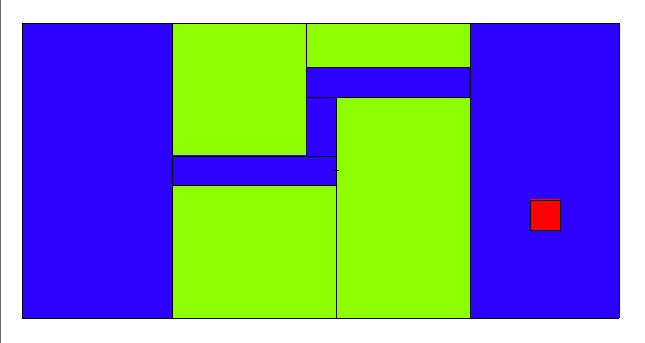
\includegraphics[width=10cm]{./chapters/characterization_probs/figures/geometries/maze2.png}
  \caption[Single turn labyrinth geometry.]{Single turn labyrinth geometry.}
  \label{fig:maze2geom}
\end{figure}

\begin{figure}[h!]
  \centering
  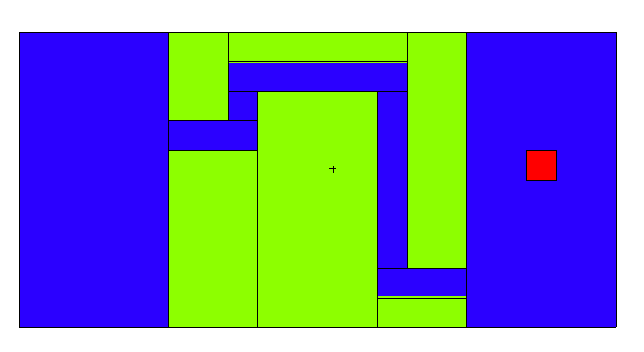
\includegraphics[width=10cm]{./chapters/characterization_probs/figures/geometries/maze1.png}
  \caption[Multi-turn labyrinth geometry.]{Multi-turn labyrinth geometry.}
  \label{fig:maze1geom}
\end{figure}

\subsubsection*{Steel beam in Concrete}

\begin{figure}[h!]
  \centering
  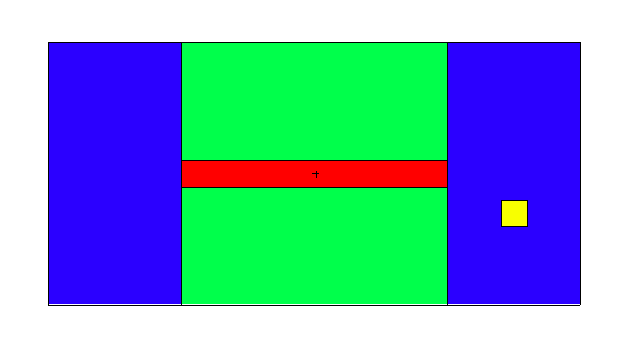
\includegraphics[width=12cm]{./chapters/characterization_probs/figures/geometries/prob-1.png}
  \caption[Steel plate embedded in concrete.]{Steel plate embedded in concrete.}
  \label{fig:prob1geom}
\end{figure}

Figure \ref{fig:prob1geom} is a variant problem with a steel beam embedded in
concrete. A NaI detector is located on the right hand side of the problem to
record the response in CADIS problems. The source is a 80x80 centimeter
sheet pointed in
towards the steel structure in the $+x$ direction emitting 10 MeV neutrons.
Because the particles have preferential flow through the steel but do do not
have long streaming paths, this problem has material heterogeneity and will be
highly scattering, but will not have streaming paths in the shielding region.
Further, because the source is emitted from a thin plate in $+x$, it is
monodirectional. This problem may have some ray effects occurring from
backscattering off of the steel and concrete in the left side air region.
It
may also have ray effects exiting the beam on the right hand side. However, because
significantly more scattering will happen in the concrete, the ray effects on
the right hand side will be less pronounced than in the air exits of the
labyrinths.

\subsubsection*{U-shaped corridor}

\begin{figure}[h!]
  \centering
  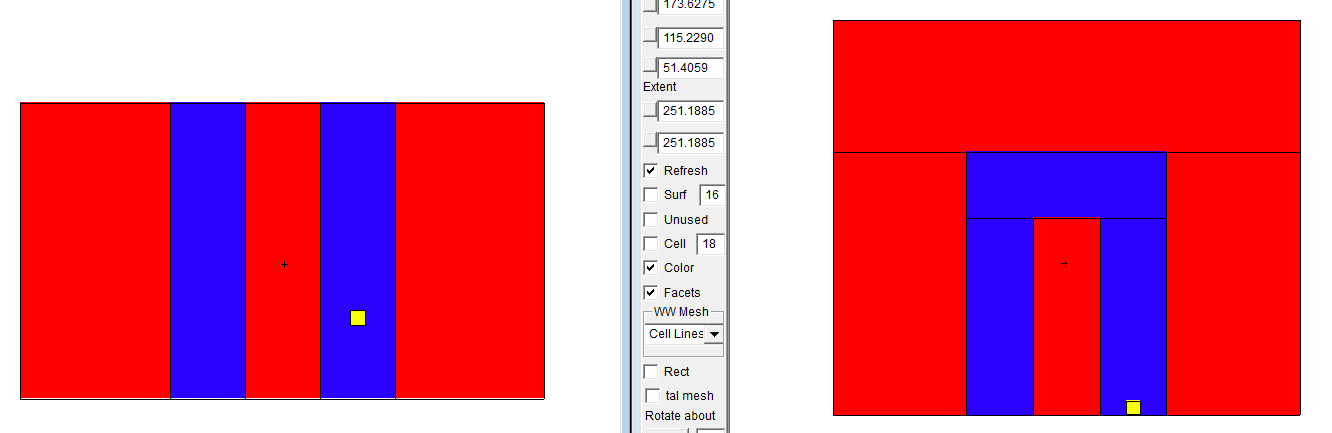
\includegraphics[width=15cm]{./chapters/characterization_probs/figures/geometries/prob-2.png}
  \caption[U-shaped corridor in concrete]{U-shaped corridor in concrete.}
  \label{fig:prob2geom}
\end{figure}

The U-shaped corridor illustrated in Figure \ref{fig:prob2geom} is somewhat
similar to the maze variants from Figs. \ref{fig:maze2geom} and
\ref{fig:maze1geom}. On the left-hand side of the corridor there is a point source
emitting a Watt spectrum of $^{235}$U neutrons. The right leg of the corridor
has a NaI detector. Without the large air voids in the labyrinth variants, the
U-shaped corridor will have
less prominent ray effects. The heterogeneity between
the air and concrete will preferentially transport particles through the air,
and particles interacting with the concrete will downscatter in energy.

\subsubsection*{Concrete shielding with rebar}

\begin{figure}[h!]
  \centering
  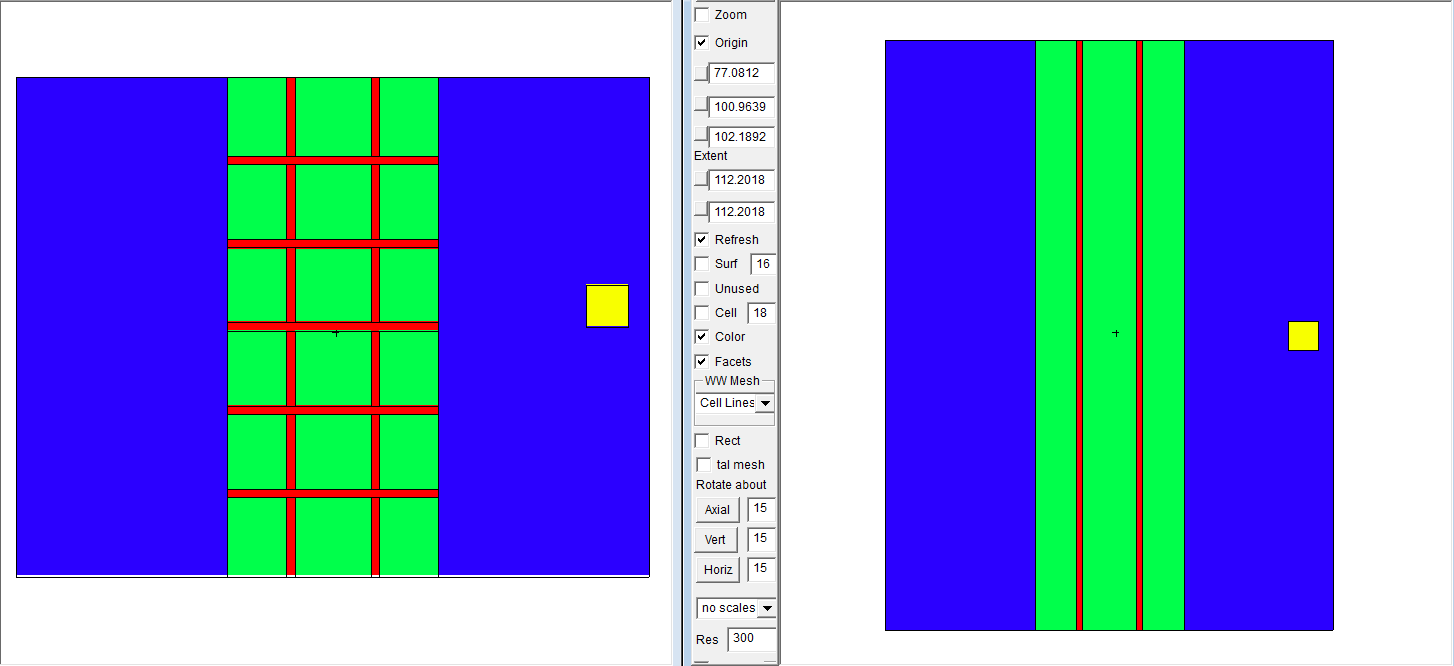
\includegraphics[width=15cm]{./chapters/characterization_probs/figures/geometries/prob-4.png}
  \caption[Concrete shielding with rebar]{Concrete shielding with rebar.}
  \label{fig:prob4geom}
\end{figure}

The shielding material illustrated in Figure \ref{fig:prob4geom} is built off of
the steel structural beam problem in Figure \ref{fig:prob1geom}. However, this is a more
realistic illustration of rebar in concrete. In this problem, a NaI detector is
used to measure the response on the right hand side of the problem in yellow.
The source is both space- and energy-dependent, emitting a Watt spectrum of
neutrons characteristic of $^{235}$U fission, and is distributed in a 100x160
centimeter plate
on the left hand side of the problem. The source is monodirectional in $+x$.
The two images provided show
different xy-plane cutaways of the shielding, with steel rebar running through
the concrete in different directions. This problem will have angular
dependence, but preferential flowpaths through the concrete are not directed
towards the detector location on the other side of the shielding in some of the
rebar. This problem has material heterogeneity both in the concrete and between
the concrete and air. This problem is highly scattering from the concrete, and
is unlikely to have ray effects without a strong single preferential flowpath
through the shield.

\subsubsection*{Nuclear medicine therapy room}

\begin{figure}[h!]
  \centering
  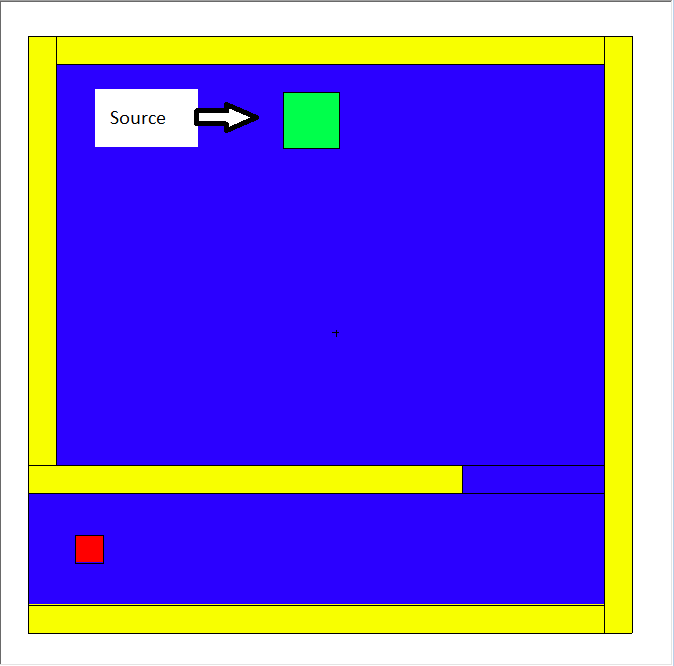
\includegraphics[height=8cm]{./chapters/characterization_probs/figures/geometries/therapy-room.png}
  \caption[Nuclear medicine therapy room.]{Therapy room geometry.}
  \label{fig:therapygeom}
\end{figure}

A small application problem relevant to the interests of this project is the
therapy room illustrated in Figure \ref{fig:therapygeom}. This room has concrete
walls, a water-based phantom that is being irradiated by a monodirectional
source in the room, and a hallway where a therapy technician might walk. In a
CADIS run of this problem, we seek to calculate the response in the
technician in the hallway from particles that are not absorbed by the patient in
the room. Because this problem is primarily air with concrete
borders, it will have strong streaming effects in the air. Particles that do
make it to the technician will be produced by emission from the patient in the
room, by scattering off air or by scattering off walls.
Because of the high fraction of air in this problem, we also anticipate
ray effects to occur. While there will be scattering in this problem, it will
not be as strong of an effect as other characterization problems.

Now that the broad subset of characterization problems have been described,
the physics that each contains is summarized in Table \ref{tab:probphysics}.
The table illustrates that it is difficult to separate one cause of flux
anisotropy from another in a characterization problem. This is
especially true in generating a problem that has ray effects without streaming
paths, and in constructing a highly scattering problem that has preferential
flow paths but does not have material heterogeneity. This is a
deficiency of the characterization problem construction, and is certainly an
area that may be improved upon in future work.

\begin{table}[h!]
  \centering
  \begin{tabular}{l|C{2cm}C{2cm}C{2cm}C{2cm}C{2cm}}
% \begin{tabular}{l|ccccc}
\toprule
\multirow{2}{*}{Problem Name} &  \multicolumn{4}{c}{Problem Coverage} \\
{} &  Streaming Paths & Highly Scattering & Material Heterogeneity &
Monodirectional Source & Ray \newline Effects \\
\midrule
Beamline              & x &   &   & x & x \\
Maze variants         &   &   &   &   &   \\
\textit{Single turn}  & x & x & x &   & x \\
\textit{Multi-turn}   & x & x & x &   & x \\
Steel plate           &   & x & x & x & x$^{\dagger}$  \\
U-shaped corridor     & x & x & x &   &   \\
Shielding with rebar  &   & x & x & x &   \\
Therapy Room          & x &   & x & x & x \\
\bottomrule
\end{tabular}
\begin{flushleft}
\footnotesize{
  $^{\dagger}$ May have ray effects in low density region exiting the metal
  plate, but effects will be less pronounced than other problems.
}
\end{flushleft}

  \caption[Anisotropy-inducing physics of each of the characterization problems.]
  {Anisotropy-inducing physics of each of the characterization problems.
  Each identified anisotropy-inducing physical metric is used in different
  combinations for the characterization problems. This will help to aid in
  extrapolating to which real problems the $\Omega$-methods may be applied.}
  \label{tab:probphysics}
\end{table}
% maybe it would be worthwhile to add a table of source definitions between each
% of the char problems. Some of them are monoenergetic, some are
% monodirectional, and some are monospatial(?) (point sources). A table would be
% a good way to summarize this information.

\subsection{Introduction to Data Visualization and Analysis}
\label{subsec:resultsintro}

At this point several characterization problems have been identified for their
properties in inducing anisotropy in the particle flux.
Prior to going through the results for each of the characterization problems,
this section shows how the data for each problem is presented and
walks through the reasoning behind this approach to the analysis. This
starts with example tables and figures of the FOM and tally results.
Then, plots explaining the anisotropy metrics follow. This is
accompanied by a
discussion about how the anisotropy metrics can be
related to the FOM and the relative error.

\subsubsection*{Figure of Merit and Timing Tables}

In Section \ref{sec:FOMvariants} several equation variants of
the FOM were
presented as quantifications of method success. The FOMs for each
characterization problem are presented in tabular form, similar to Table
\ref{tab:fom_defaults}. As discussed in that section, the FOM is dependent on
the relative error and the time to obtain that relative error. For the hybrid
cases, six different FOMs will be presented: three FOMs based on the tally average
relative error, the tally maximum relative error, and the tally minimum relative
error, and two FOMs based on the Monte Carlo runtime and the hybrid runtime. The
unbiased analog Monte Carlo does not have a deterministic runtime, so only the
three FOM variants based on the relative error are presented for those runs.
When analyzing the results in the FOM table for each characterization problem,
consider that the tally average relative error is calculated from all
particles contributing to all tally bins in the problem. Thus the FOM reported
for the tally average relative error may be outside of the bounds of the tally
minimum or the tally maximum relative error.
Table \ref{tab:fom_defaults} summarizes which
equations were used to calculate each FOM; each equation number is noted
in brackets.

\begin{table}[h!]
  \centering
  \begin{tabular}{l|m{3.5cm}m{3.5cm}m{3.5cm}}
\toprule
{} &   \multicolumn{2}{c}{CADIS or CADIS-$\Omega$}   & analog \\
{FOM Variant} &   MC \eqref{eq:FOMMC} & MC$_{hybrid}$ \eqref{eq:FOMHybrid} &  MC \\
\midrule
tally avg \eqref{eq:FOMavg}  &  FOM$_{avg,MC}$ &   FOM$_{avg,hybrid}$   & FOM$_{avg,MC}$   \\
max RE  \eqref{eq:FOMmax}    &  FOM$_{max,MC}$  &   FOM$_{max,hybrid}$  &  FOM$_{min,MC}$ \\
min RE      &   FOM$_{min,MC}$  &   FOM$_{min,hybrid}$   &  FOM$_{min,MC}$ \\
time (mins) & T$_{MC}$ & T$_{hybrid}$ \eqref{eq:hybridtime} &  T$_{MC}$ \\
\bottomrule
\end{tabular}

  \caption[Table of FOM variants used to measure $\Omega$-method performance.]{
  Table of FOM variants used to measure $\Omega$ performance. Relevant equations
  can
  be found in Section \ref{sec:FOMvariants} and are referenced in the table in
  parentheses.}
  \label{tab:fom_defaults}
\end{table}

Tables calculating the FOMs summarized in Table \ref{tab:fom_defaults} may
not have evaluated FOMS in some locations. These will be noted with a dashed
line, or ``--''.  These values will generally be in the minimum relative error
section of the FOM tables, and they represent a zero relative error. This
does not mean that infinite particles have been sampled (so the relative error
is infinitely small), but rather that no particles have been binned for that
energy bin.
This technically results in an infinite FOM, but in reality
represents a bin that will never converge. Because this value will hold no
meaning in our quantification of the $\Omega$-methods' success, the infinite
valued FOM is not included.


Table \ref{tab:time_defaults} reports the times used to calculate the
FOM values in Table \ref{tab:fom_defaults} more detail. This table is
split into three
vertical regions: the MCNP time spent doing Monte Carlo transport (T$_{MC}$),
the deterministic time spent in ADVANTG/Denovo (T$_{det}$),
and the walltime (T$_{hybrid}$), which is the
summation of the two. The deterministic time section contains
further segmentations of timing. This is because processes in ADVANTG are
run using different computational resources. ADVANTG itself is a driver script
that can launch a paralellized run in Exnihilo/Denovo, but it also postprocesses the
Denovo fluxes into source biasing and weight window parameters. The processes
exclusive to ADVANTG, like generating the biasing parameters, are performed in
serial on a single processor. Conversely, all of the Denovo calculation is run
in parallel on any number of cores specified by the user. To ensure that a
comparable time is used when calculating the adjusted FOM, we have chosen to
calculate the total walltime spent in each calculation. Thus, the parallelized
clock time is multiplied by the total number of cores to obtain T$_{denovo}$.
This quantity is summed with
the runtimes of the other serial tasks to obtain the total deterministic runtime.

\begin{table}[h!]
  \centering
  \begin{tabular}{L{2.5cm}L{3cm}C{3cm}C{4cm}C{2cm}}
\toprule
          &              &          CADIS &   CADIS-$\Omega$ &         analog \\
          &              & time (minutes) & time (minutes)   & time (minutes) \\
\midrule
MCNP time &  total (T$_{MC}$) &         T$_{MC,cad}$ &     T$_{MC,cad-\Omega}$ & T$_{MC,analog}$  \\
deterministic time & advantg time (T$_{adv}$) &           0.18 &           0.18 &            -- \\
    & denovo time (T$_{denovo}$) &           5.69   &          25.64 &            -- \\
                   & dispose time &           0.00  &           0.16 &            -- \\
                   & omega time (T$_{\Omega}$)&    --      &           0.66 &            -- \\
                   & total (T$_{det}$) &  T$_{adv}$+T$_{denovo}$  &
                   T$_{adv}$+T$_{denovo}$+T$_{\Omega}$ &            -- \\
wall time & total (T$_{hybrid}$) &  T$_{MC,cad}$ + T$_{det,cad}$ &  T$_{MC,cad-\Omega}$ + T$_{det,
cad-\Omega}$ &  T$_{MC,analog}$  \\
\bottomrule
\end{tabular}

  \caption[Table of differing times used to measure $\Omega$ performance.]{
    Table of differing times used to measure $\Omega$ performance. These times
    are used to calculate the FOMS in Table \ref{tab:fom_defaults}. }
  \label{tab:time_defaults}
\end{table}

Two other times are listed under the deterministic time that may or may not be
included in T$_{hybrid}$, which are T$_{\Omega}$ and T$_{dispose}$. T$_{dispose}$ is the
reported times that are not included in the calculation of T$_{det}$ in either
CADIS or CADIS-$\Omega$. It is a sum of time results that either are not
important to comparing the methods--like calculating the anisotropy metrics--or
times that are accounted for by other tasks in T$_{det}$. This prevents overlap
of times and provides a more realistic comparison between the performance of
both methods.

The reported $\Omega$ time, T$_{\Omega}$, is the total
time spent in the tasks unique to the $\Omega$-methods. This includes reading
in the angular flux files, performing the computation of Eq.
\eqref{eq:omega_basic}, and writing the $\Omega$-results to a file.
The $\Omega$ time,
though run in Denovo, is still a serial calculation so is separated out from the
total Denovo time. The $\Omega$-method tasks at this time are not
parallelized, so the clock time is treated in the same way as the reported
ADVANTG time. Because the majority of the $\Omega$-flux generation
infrastructure is implemented in Exnihilo rather than ADVANTG, future expansions
of the method could be parallelized for faster clock times.

Because the adjusted FOM (the FOMs labeled FOM$_{hybrid}$ in Table
\ref{tab:fom_defaults}) uses T$_{Hybrid}$, which is the total runtime of the
Monte Carlo calculation (T$_{MC}$) and the hybrid/deterministic run preceding it
(T$_{det}$), it will differ between
the $\Omega$-methods, standard CADIS, and standard FW-CADIS.
For CADIS, T$_{det}$ is
the sum of the ADVANTG runtime and the wall time of the Denovo transport. For
CADIS-$\Omega$, this is the sum of the ADVANTG runtime, the wall time of the
Denovo transport, and the time spent in the $\Omega$-flux calculation. How each
time is calculated is summarized in Table \ref{tab:time_defaults}.

Beyond
adding the $\Omega$-flux compute time, CADIS-$\Omega$ will generally have much
longer Denovo runtimes than CADIS. This is a combination of the $\Omega$-methods'
requirement of both a forward and adjoint calculation (recall that CADIS
requires only the adjoint calculation), and that the $\Omega$-methods require
full angular flux solutions to calculate the $\Omega$-flux. While standard CADIS
has the ability to print the full angular flux solutions as CADIS-$\Omega$, it
is neither a requirement nor is it standard practice. The I/O demands to both write
the angular fluxes and then read them back in is a potential bottleneck in the
method based on the current implementation.

\subsubsection*{Tally Result and Relative Error Plots}

Each of the problems introduced in Section \ref{subsec:ProbSpecs} has a
10x10x10 cm detector in which the tally response is calculated. The tallies are
discretized in energy; the tally result and associated relative error are
tabulated for each energy bin. Some of this information can be inferred from Table
\ref{tab:fom_defaults},
but seeing the distribution of the relative errors for each energy
bin for each method is a useful way of seeing how effective each method is at
biasing particles all of the tally bins,
without time effects. As described in the previous paragraph, CADIS-$\Omega$'s
deterministic time will be longer than CADIS', so the FOM$_{hybrid}$ may be
lower for the $\Omega$-methods, even if the relative errors are better.
Presenting both the relative error distribution and the FOM will provide a clear
picture of the performance of the $\Omega$-methods.

The tally results and relative errors for CADIS,
CADIS-$\Omega$, and the nonbiased analog Monte Carlo will be
presented in figures similar to
\ref{fig:sampleresult} and \ref{fig:sampleerror}.
In the case where the
relative error of the nonbiased analog Monte Carlo far exceeds the errors
achieved by CADIS and CADIS-$\Omega$, it will be omitted. The example given in
Figure \ref{fig:sampleerror} shows a result where this is the case.
The hybrid methods
will be marked with a dashed line; the nonbiased analog Monte Carlo will be a
solid line.

\begin{figure}[ht!]
  \centering
  \begin{subfigure}[t]{\textwidth}
    \centering
    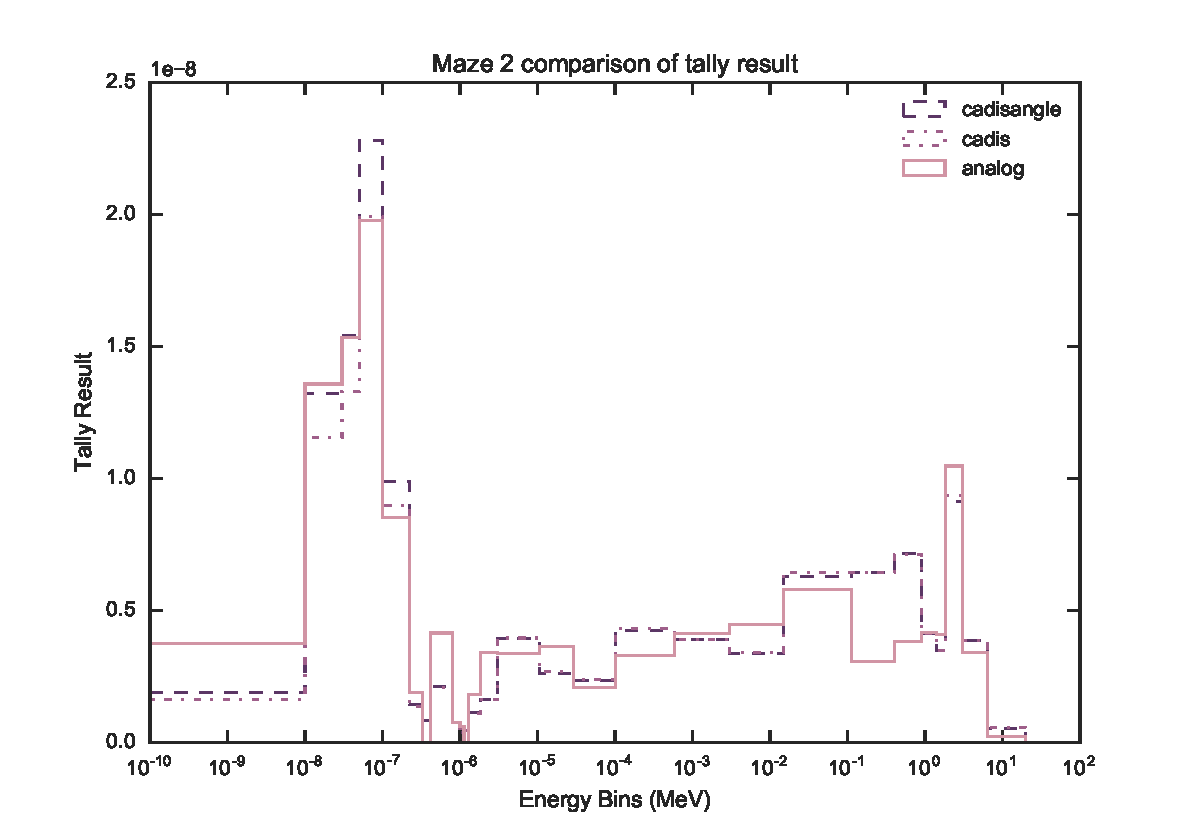
\includegraphics[width=0.8\linewidth]{./chapters/characterization_probs/figures/char/maze2/maze_2_tally_result_compare.pdf}
    \caption{Comparison between methods of the tally result.}
    \label{fig:sampleresult}
  \end{subfigure}
  \begin{subfigure}[t]{\textwidth}
    \centering
    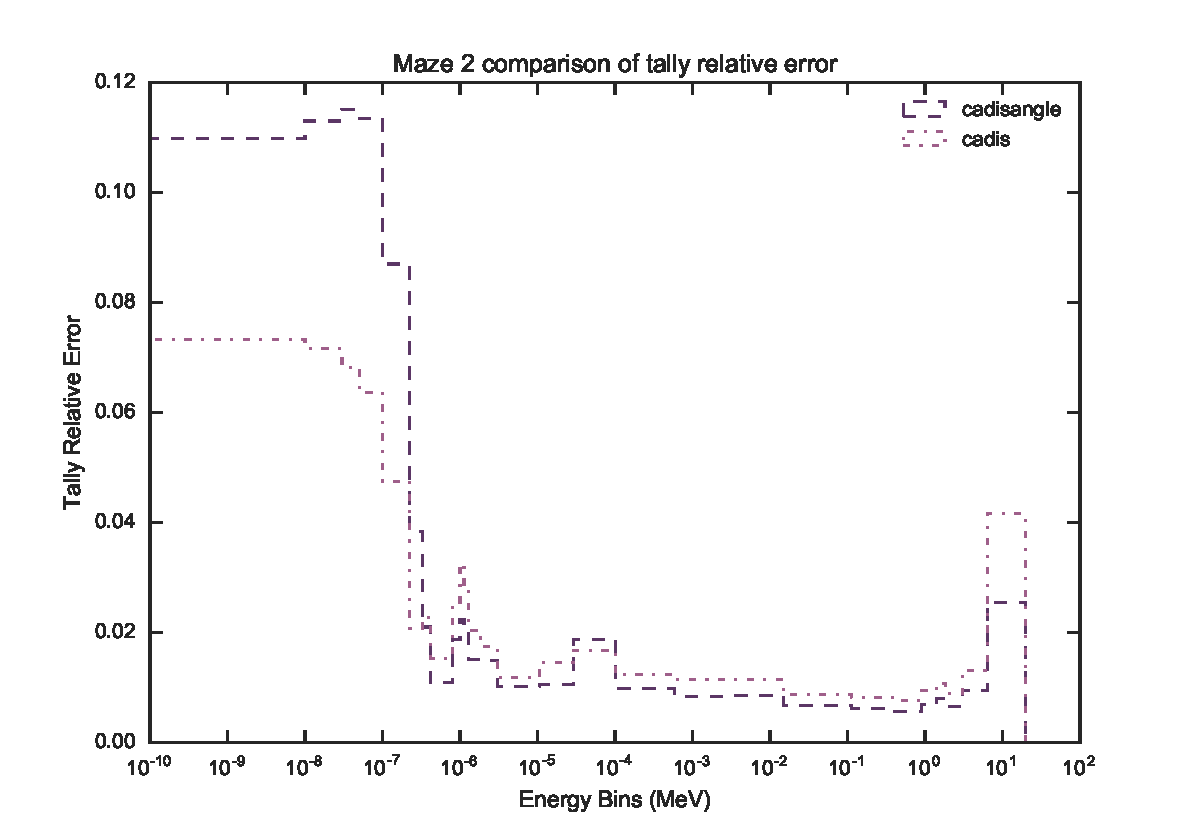
\includegraphics[width=0.8\linewidth]{./chapters/characterization_probs/figures/char/maze2/maze_2_tally_error_compare.pdf}
    \caption{Comparison between methods of the tally relative error.}
    \label{fig:sampleerror}
  \end{subfigure}
  \caption[Sample results for a characterization problem tally.]{Sample results
  for a characterization problem tally.}
\end{figure}

\subsubsection*{Anisotropy Metrics}

Equations \eqref{eq:metric_one} through \eqref{eq:metric_six} in
Section \ref{sec:anisotropy_quant} presented several different ways by which the
anisotropy of each problem could be quantified. As discussed in that section,
Each metric will show slightly differing effects. For example, the ratio of the
$\Omega$- to adjoint-flux in metric two will differ significantly from the
angular contributon max to average of metric three. The $\Omega$-flux
may be larger or smaller than the adjoint scalar flux depending on the
directionality of the adjoint and forward particles relative to one another. If
the particles are travelling in opposite directions, this will result in a
larger omega flux than the adjoint flux. If they stream in the same direction
(away from the tally detector, for example),
then the resultant $\Omega$ flux will be smaller than the adjoint. In the case
of the angular contributon max to average the distribution will have a lower
limit where the maximum is very close to the average contributon flux. It can
never be lower than the average. In a isotropic problem, the majority of the
cells in the problem will be this ratio, whereas in a strongly anisotropic
problem this distribution will shift upwards, but will still have the same
limiting lower value as the isotropic case.

\begin{figure}[htb!]
  \centering
  \begin{subfigure}[t]{\textwidth}
    \centering
    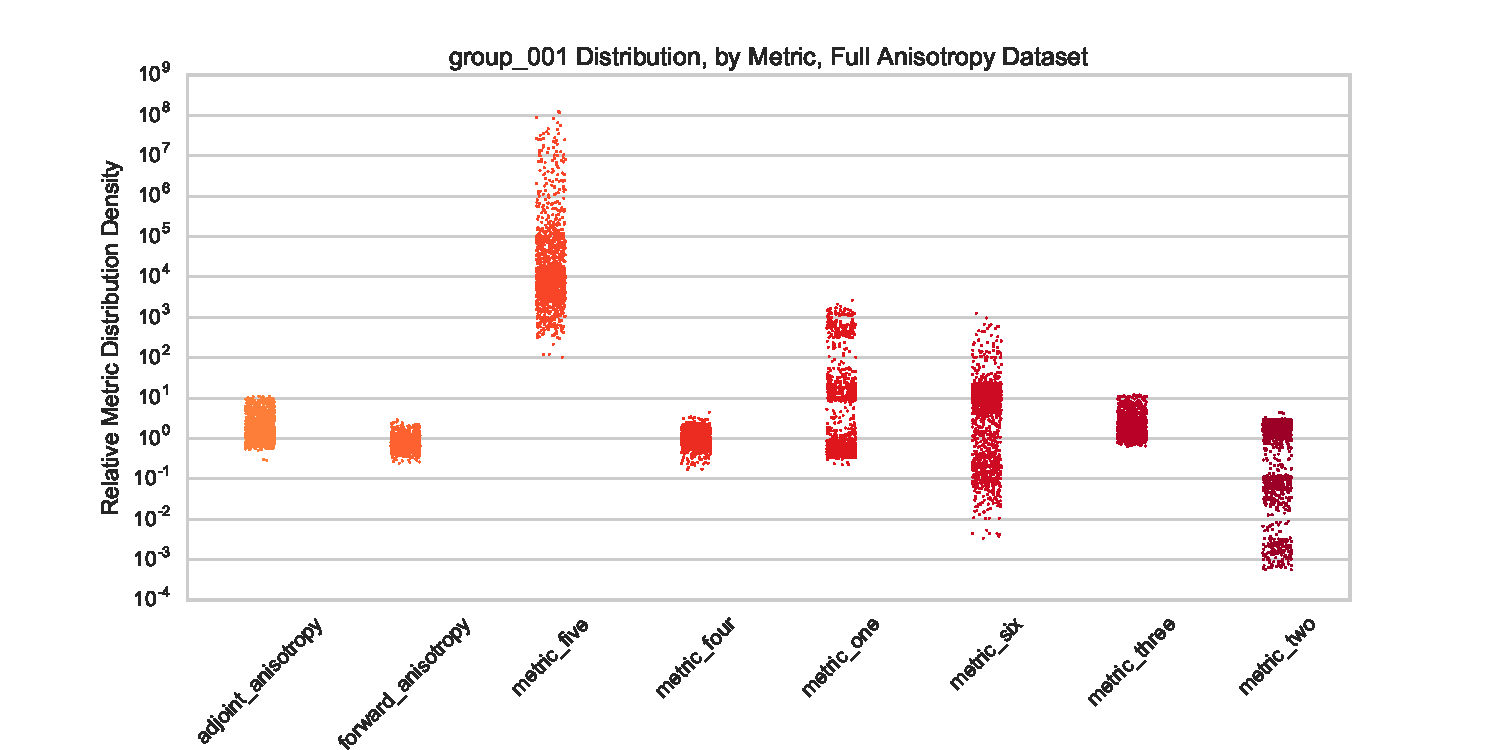
\includegraphics[width=0.95\linewidth]{./chapters/characterization_probs/figures/sample_data/group_001_strip_full.pdf}
    \caption{Example distribution of anisotropy metrics for fastest energy group.}
    \label{fig:samplestrip001}
  \end{subfigure}
  \begin{subfigure}[t]{\textwidth}
    \centering
    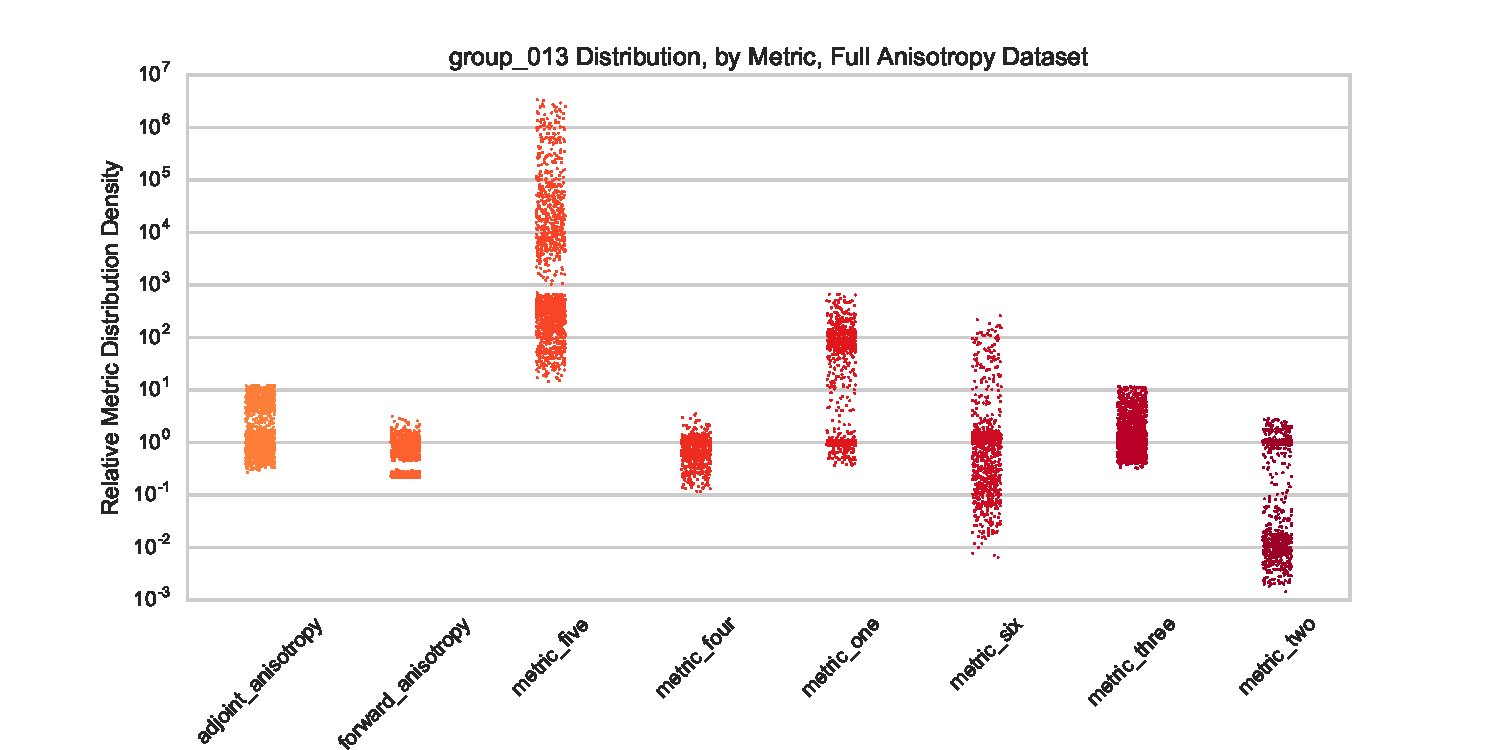
\includegraphics[width=0.95\linewidth]{./chapters/characterization_probs/figures/sample_data/group_013_strip_full.pdf}
    \caption{Example distribution of anisotropy metrics for epithermal energy group.}
    \label{fig:samplestrip013}
  \end{subfigure}
\end{figure}
\begin{figure}[htb!]\ContinuedFloat
  \begin{subfigure}[t]{\textwidth}
    \centering
    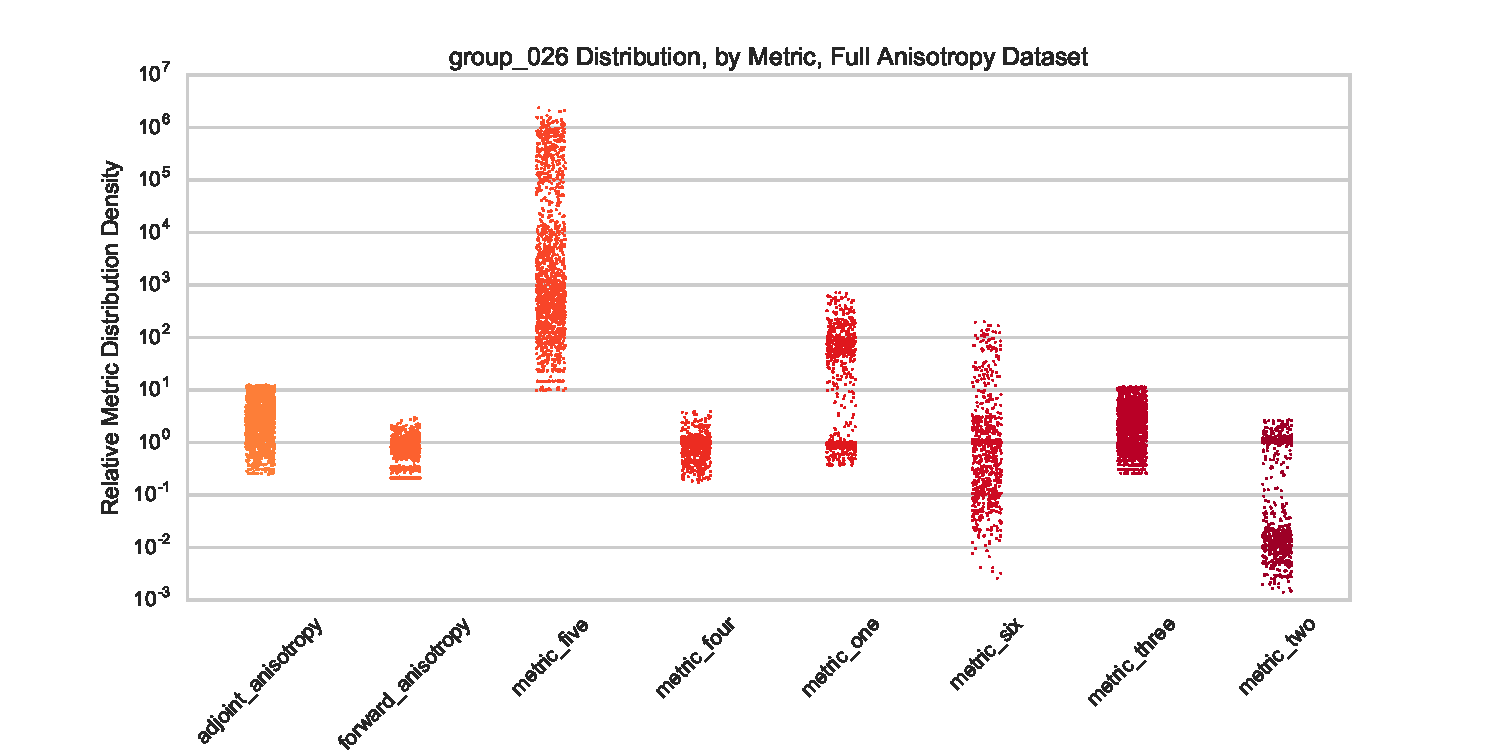
\includegraphics[width=0.95\linewidth]{./chapters/characterization_probs/figures/sample_data/group_026_strip_full.pdf}
    \caption{Example distribution of anisotropy metrics for thermal energy group.}
    \label{fig:samplestrip026}
  \end{subfigure}
  \caption[Example distribution of all anisotropy metrics for highest,
  intermediate, and lowest energy groups.]{Example distribution of all
  anisotropy metrics for highest, intermediate, and lowest energy groups.}
  \label{fig:samplestrips}
\end{figure}

To illustrate the effect of how different the anisotropy metrics' distributions
are, Figure \ref{fig:samplestrips} shows stripplots for all of the anisotropy
metrics for three different energy groups in one of the characterization
problems. The effects of thermalization--and consequently more induced
isotropy--on each of the metrics can be seen clearly as one
scans from Fig \ref{fig:samplestrip001} to \ref{fig:samplestrip026}.

The adjoint
anisotropy metric, the forward anisotropy metric, and metric three are all
shifted by a factor of $4\pi$. Their natural lowest limit should be near unity
but all lie lower. This may be corrected in the future, but for the
purposes of this analysis we are more interested in the relative distribution
and the consistent factor of $4\pi$ is not important to that effect.

A stripplot shows distinct data points, but easily can be overwhelmed if the
full number of cells is used in a single strip. The figures in
\ref{fig:samplestrips} contain a random selection of 1500 data points from the
full anisotropy datasets,
which is only a small fraction of the number of cells in the characterization
problem meshes. There are other ways to visualize the full distribution of the
dataset. Figure \ref{fig:sampledistros} shows three modes
by which an anisotropy metric can be visualized.
These plots, unlike Figure \ref{fig:samplestrips}, show a
single metric but all energy groups. The highest/fastest energy group
is plotted in deep red, and the lowest or most thermal
energy group is shown in blue.

\begin{figure}[htb!]
  \centering
  \begin{subfigure}[t]{\textwidth}
    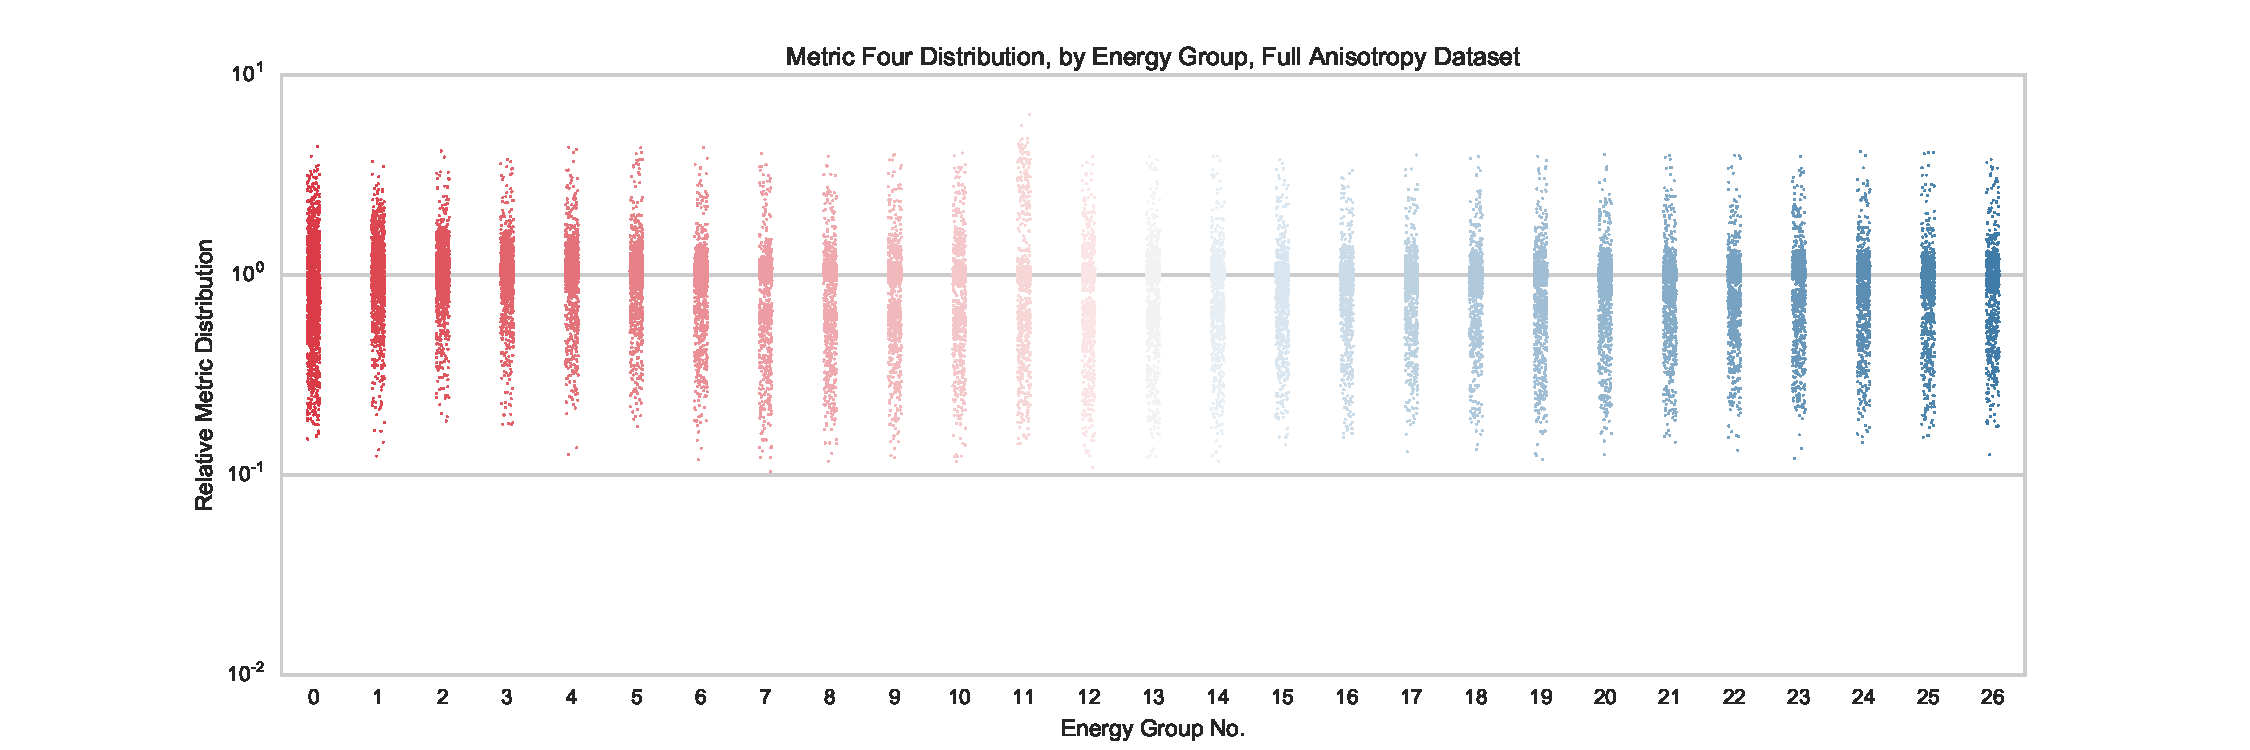
\includegraphics[width=\linewidth]{./chapters/characterization_probs/figures/sample_data/metric_four_strip_full.pdf}
    \caption{Example distribution of M$_4$, all energy groups, strip plot.}
    \label{fig:samplestripM4}
  \end{subfigure}
\end{figure}
\begin{figure}[htb!]\ContinuedFloat
  \centering
  \begin{subfigure}[t]{\textwidth}
    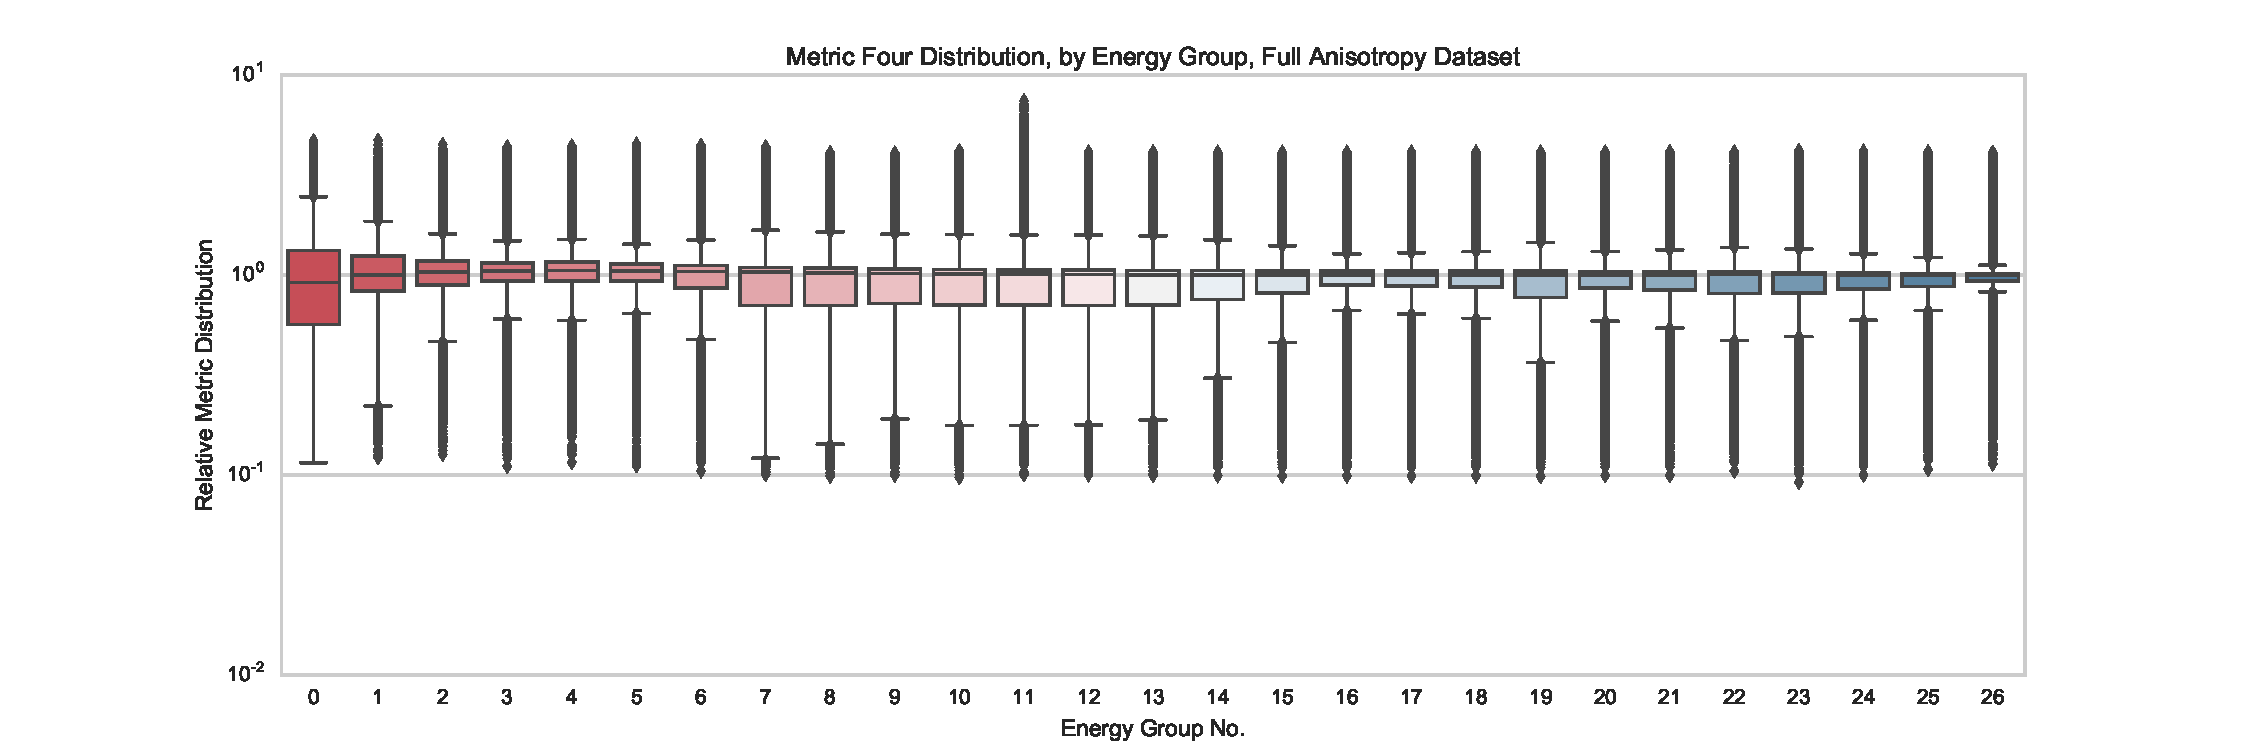
\includegraphics[width=\linewidth]{./chapters/characterization_probs/figures/sample_data/metric_four_box_full.pdf}
    \caption{Example distribution of M$_4$, all energy groups, box plot.}
    \label{fig:sampleboxM4}
  \end{subfigure}
  \begin{subfigure}[t]{\textwidth}
    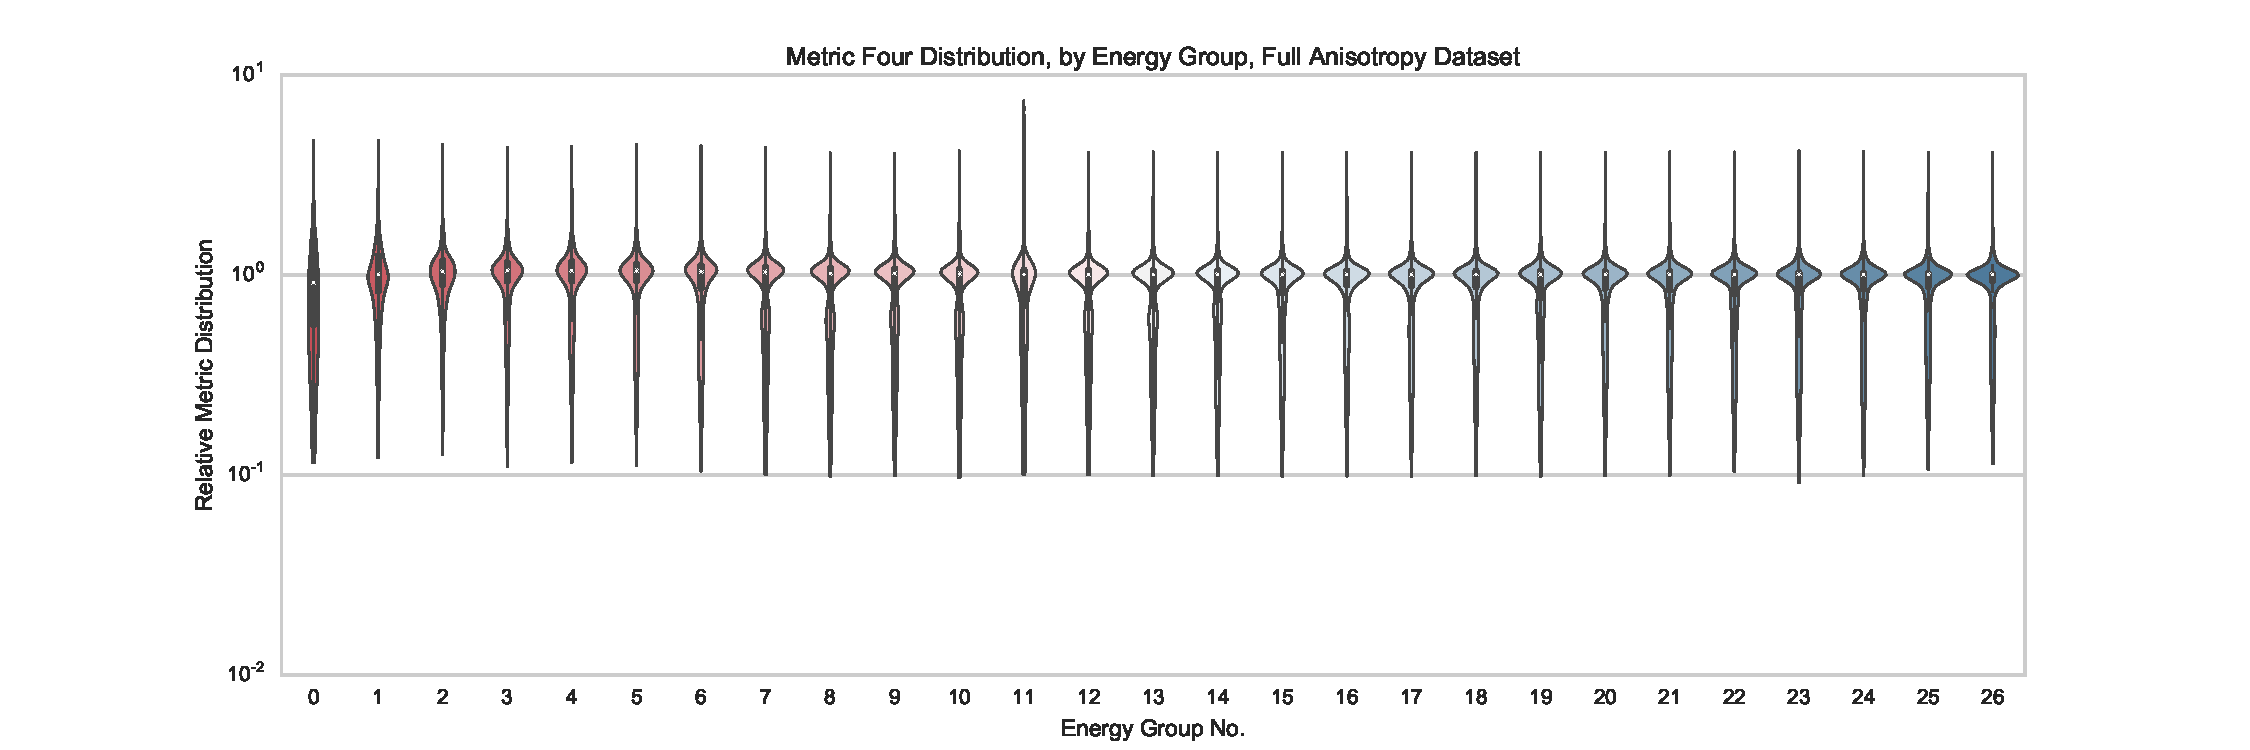
\includegraphics[width=\linewidth]{./chapters/characterization_probs/figures/sample_data/metric_four_violin_full.pdf}
    \caption{Example distribution of M$_4$, all energy groups, violin plot.}
    \label{fig:sampleviolinM4}
  \end{subfigure}
  \caption[Different ways of visualizing M$_4$ for a characterization problem.]
  {Different ways of visualizing M$_4$ for a characterization problem.}
  \label{fig:sampledistros}
\end{figure}

All three subfigures in \ref{fig:sampledistros} show the effects of
thermalization on the chosen metric distribution and density. The stripplot of
\ref{fig:samplestripM4} is a clear representation of the density, but not much
more can be ascertained about the distribution of the metric. Figure
\ref{fig:sampleboxM4} has box and whisker plots that show the data quartiles,
the mean, and outliers. However, in the case where the distribution is heavily
towards a limiting value, the mean is hard to separate from the distribution.
Further, no data on how the metric is distributed beyond the quartile markers is
provided. The violin plot of Figure \ref{fig:sampleviolinM4} is a hybrid of the
former two plots. The width of the violin is related to the density of values,
but inside the violin the limits of the box plots are marked in black. The
violin limits extend to the outliers.

The analysis for each of the characterization problems look at the result for
the tally average relative error, the tally maximum relative error, and the
tally minumum relative error. Because we are interested in how the relative
error in each energy bin changes with respect to CADIS-$\Omega$ and CADIS, the
plots showing the distributions over all energy groups for a single metric
is generally more applicable than the plots for a single energy group
but with all metrics. As a result,
future plots of the metrics will be in the style of those
in Figure \ref{fig:sampledistros} rather than \ref{fig:samplestrips}.

\subsubsection*{Filtered Anisotropy Metrics}

\begin{figure}[htb!]
  \centering
  \begin{subfigure}[t]{\textwidth}
    \centering
    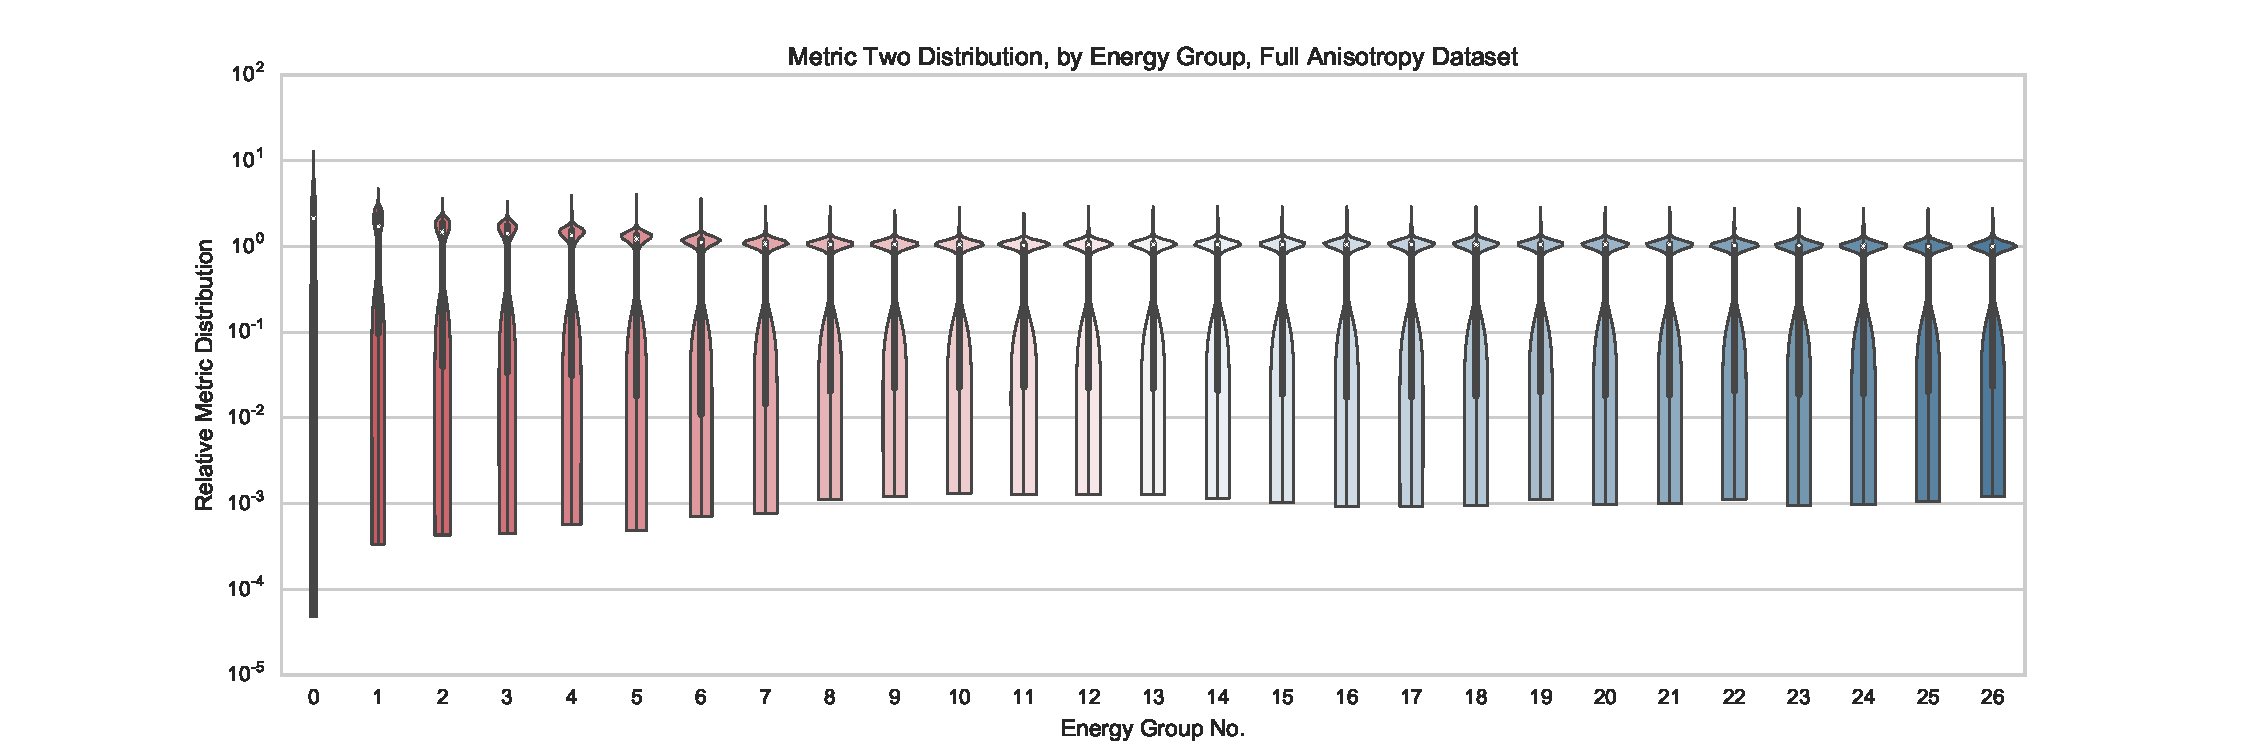
\includegraphics[width=\linewidth]{./chapters/characterization_probs/figures/sample_data/metric_two_violin_full.pdf}
    \caption{Example distribution of M$_2$, all energy groups, violin plot}
    \label{fig:samplefullviolinM2}
  \end{subfigure}
\end{figure}
\begin{figure}[htb!]\ContinuedFloat
  \centering
  \begin{subfigure}[t]{\textwidth}
    \centering
    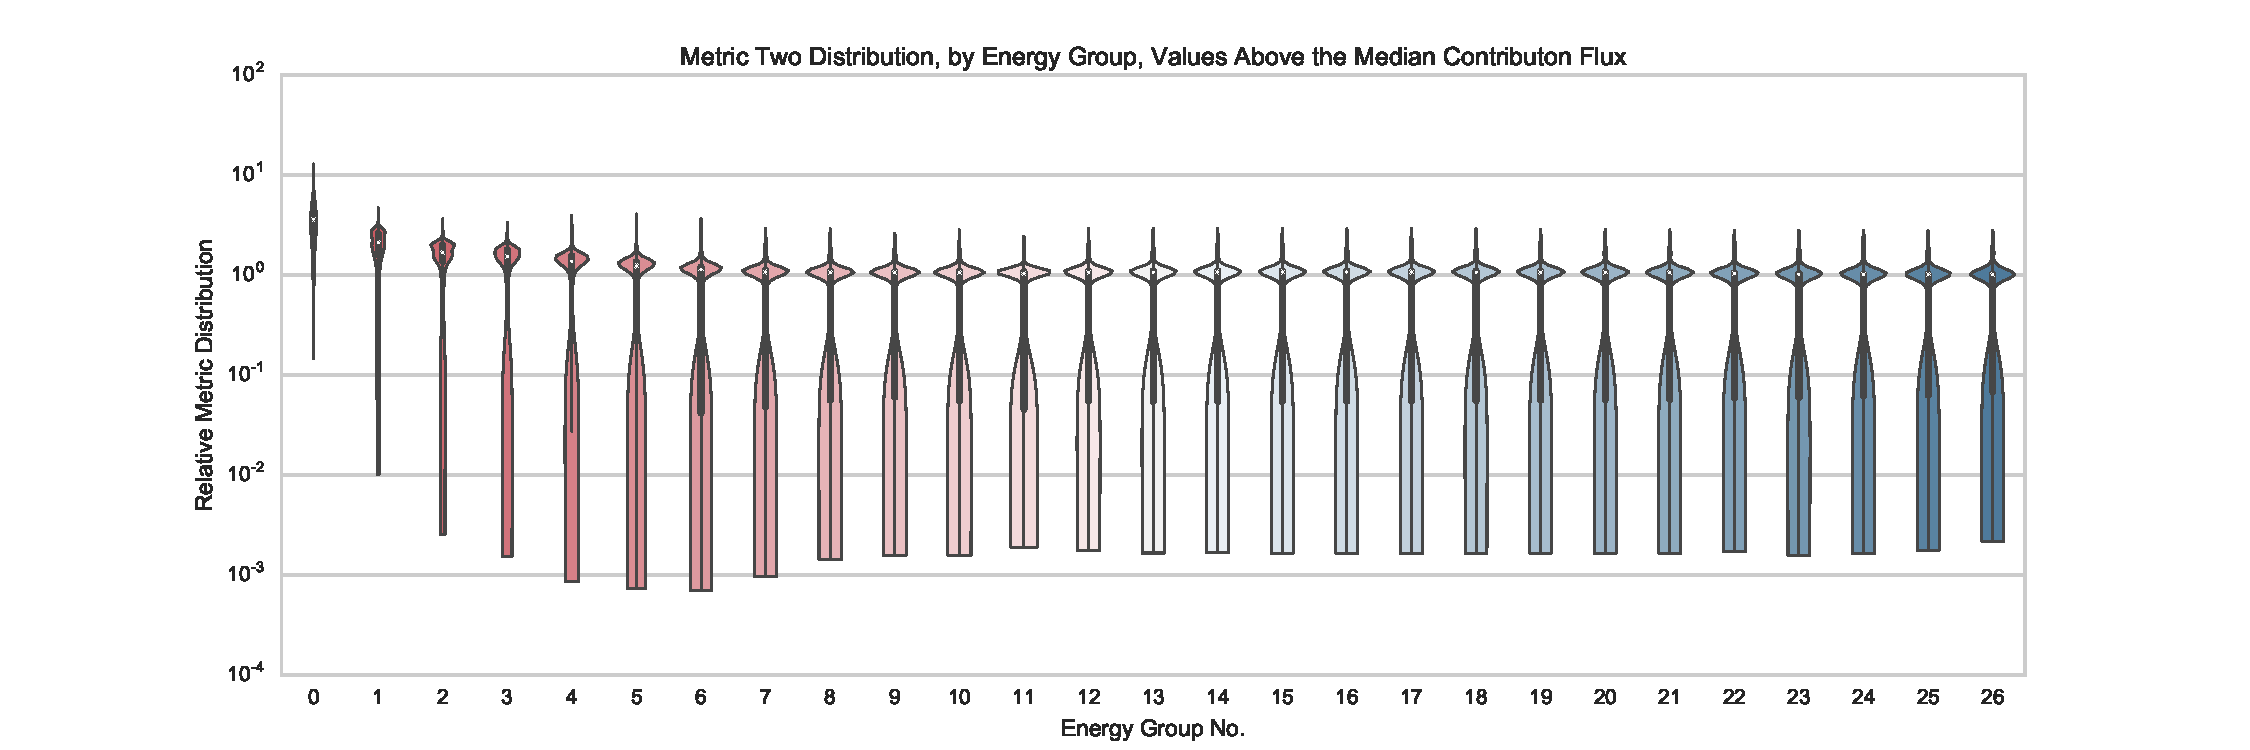
\includegraphics[width=\linewidth]{./chapters/characterization_probs/figures/sample_data/metric_two_violin_median.pdf}
    \caption{Example distribution of M$_2$, all energy groups, violin plot using
    only datapoints above the median metric value in each energy group.}
    \label{fig:samplemedianviolinM2}
  \end{subfigure}
\end{figure}
\begin{figure}[htb!]\ContinuedFloat
  \centering
  \begin{subfigure}[t]{\textwidth}
    \centering
    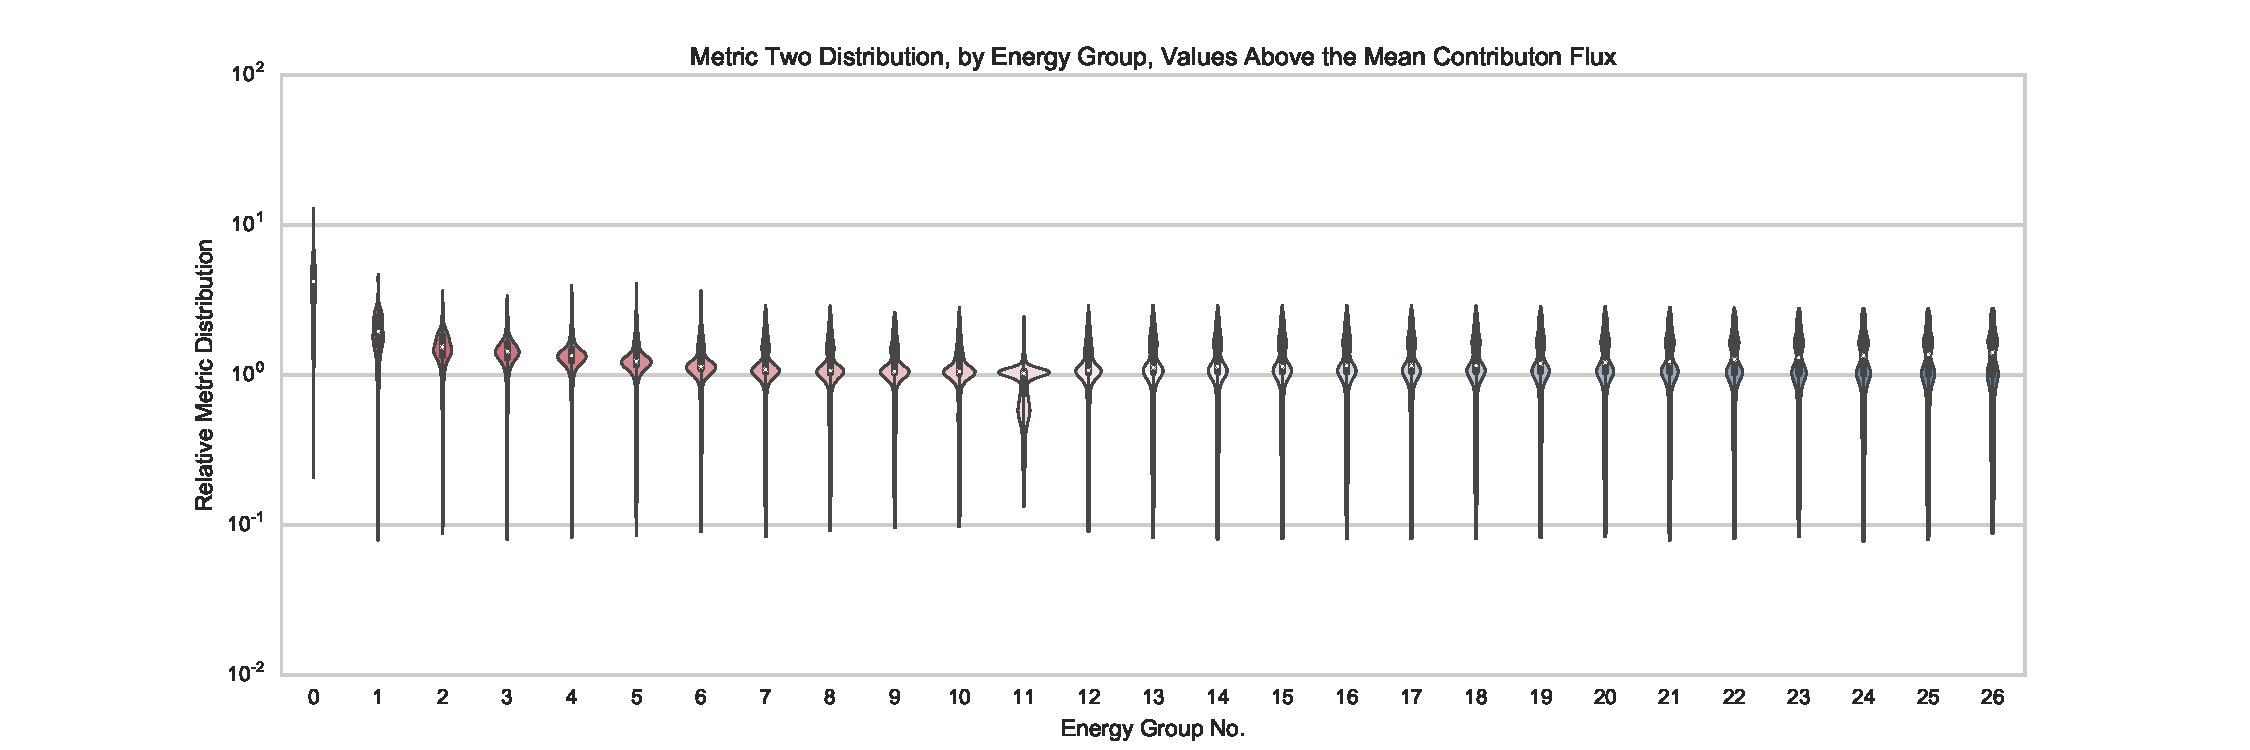
\includegraphics[width=\linewidth]{./chapters/characterization_probs/figures/sample_data/metric_two_violin_mean.pdf}
    \caption{Example distribution of M$_2$, all energy groups, violin plot using
    only datapoints above the mean metric value in each energy group.}
    \label{fig:samplemeanviolinM2}
  \end{subfigure}
  \caption[M$_2$ violin plots using different selections of the metric data.]
  {M$_2$ violin plots using different selections of the metric data.}
  \label{fig:sampleviolinsM2}
\end{figure}

Beyond plotting the anisotropy metrics as a function of energy group, we are
interested in how the relative error or FOM will respond as a function of each
metric. However, not all cells in the problem are as important as others to
contributing to the tally. A cell on the problem boundary is very unlikely to
contribute to the tally result when compared to a cell next to the adjoint
source. As discussed in Section \ref{sec:ContributonImportance}, the contributon
flux measures the response importance of a cell. By selectively choosing
anisotropy metrics from cells that are likely to induce a response, some of the noise
of less important cells can be cut out.

To consistently cut out the same number of datapoints across all metrics, we
have chosen to use a filtering algorithm based on the contributon flux in each
cell. The first filter is choosing metric values from cells where the
contributon flux is above the problem median contributon flux. This median is
evaluated separately for each energy group to ensure that the same number of
cells in each group is plotted. The second filter is choosing metric values from
cells where the contributon flux is above the problem mean contributon flux.
Again, the mean is computed separately for each energy group such that energy
groups with higher contributon fluxes do not cut out important flux values from
a different energy group. However, unlike the median filter a different number
of cells for each energy group will be filtered. This is dependent on the skew
between the contributon mean and median value for each energy group.
Because the filter is evaluated based on the
contributon flux, it can be applied to each metric consistently, meaning that
the same number of cells are filtered out between different metrics.

Figure \ref{fig:sampleviolinsM2} shows the effects of cutting out data from
unimportant cells on the M$_2$ distribution. The first figure in the series,
\ref{fig:samplefullviolinM2}, is the M$_2$ full distribution. As discussed
previously, M$_2$ will be above unity in cells where the foward and adjoint
angular fluxes travel in opposing directions, and will be below unity in cells
where they travel in the same direction. Very unimportant cells should be below
unity. Applying the first filter--selecting values above the contributon
median--to this distribution results in Figure \ref{fig:samplemedianviolinM2}.
The bottom tails of all of the distributions have been shortened, but still many
unimportant cells remain. This should be expected, as only half of cells have
been removed. Applying the second filter results in Figure
\ref{fig:samplemeanviolinM2}. The unimportant tails have been almost completely
removed from the M$_2$ distributions. Further, features in the metric
distribution once obviscated by the
tails are now visible.

\subsubsection*{Improvement Factor Correlations with Anisotropy}

Now that a way of visualizing the metric distributions has been presented,
we seek to find
how the metric distributions relate to the relative error or FOM for a given
problem. First, an improvement ratio for the relative error and FOM will be
defined. For the relative error it is
\begin{equation}
  I_{RE} = \frac{RE_{CADIS-\Omega}}{RE_{CADIS}}\bigg\rvert_{E_g},
  \label{eq:I-RE}
\end{equation}
and for the FOM it is
\begin{equation}
  I_{FOM} = \frac{FOM_{CADIS-\Omega}}{FOM_{CADIS}}\bigg\rvert_{E_g}.
  \label{eq:I-FOM}
\end{equation}
These will be henceforth be referred to as the relative error and FOM
improvement factors.
With this definition of the improvement in the FOM or the relative
error from CADIS to CADIS-$\Omega$, we now have a comparison between the updated
and standard methods. By relating this metric to the anisotropy metrics, we can
see how anisotropy of the problem influences the improvement in the relative
error or the FOM.

\begin{figure}[htb!]
  \centering
  \begin{subfigure}[t]{\textwidth}
    \centering
    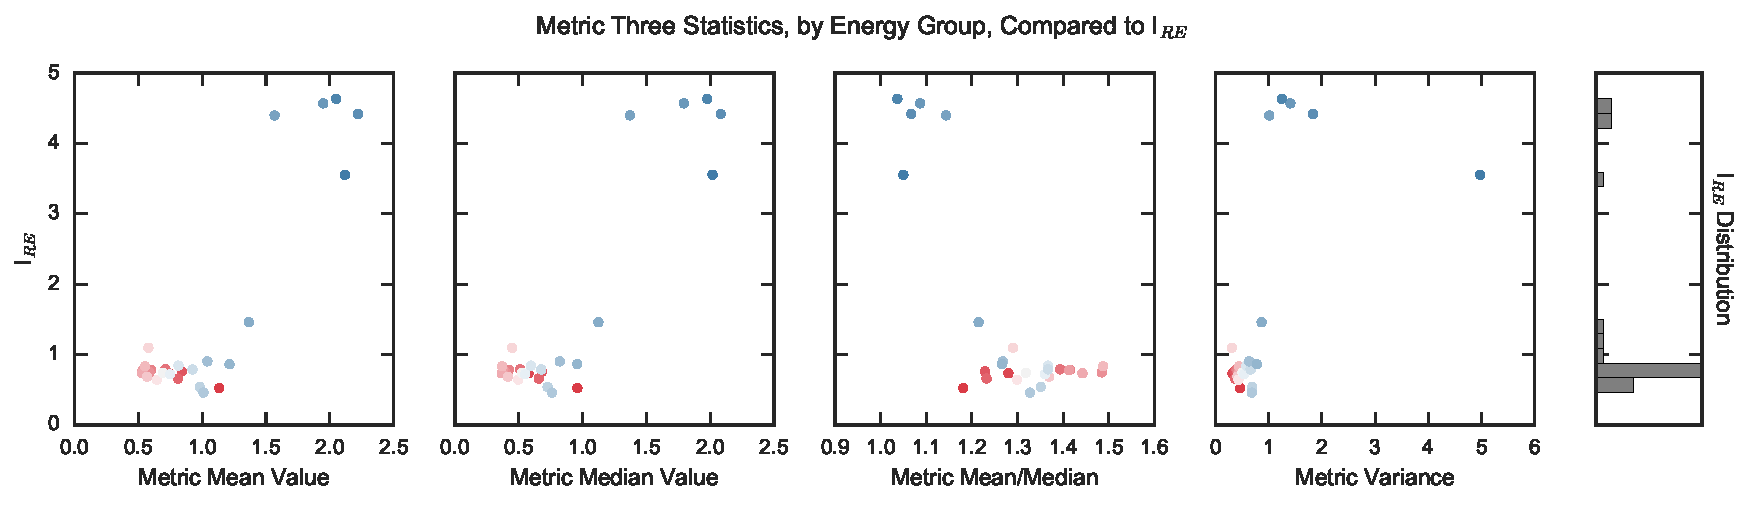
\includegraphics[width=\linewidth]{./chapters/characterization_probs/figures/sample_data/metric_three_err_stats_full.pdf}
    \caption{M$_3$ average, mean, skew, and variance plotted against the
      relative error improvement I$_{RE}$}
    \label{fig:samplestatsfullM3}
  \end{subfigure}
\end{figure}
\begin{figure}[htb!]\ContinuedFloat
  \centering
  \begin{subfigure}[t]{\textwidth}
    \centering
    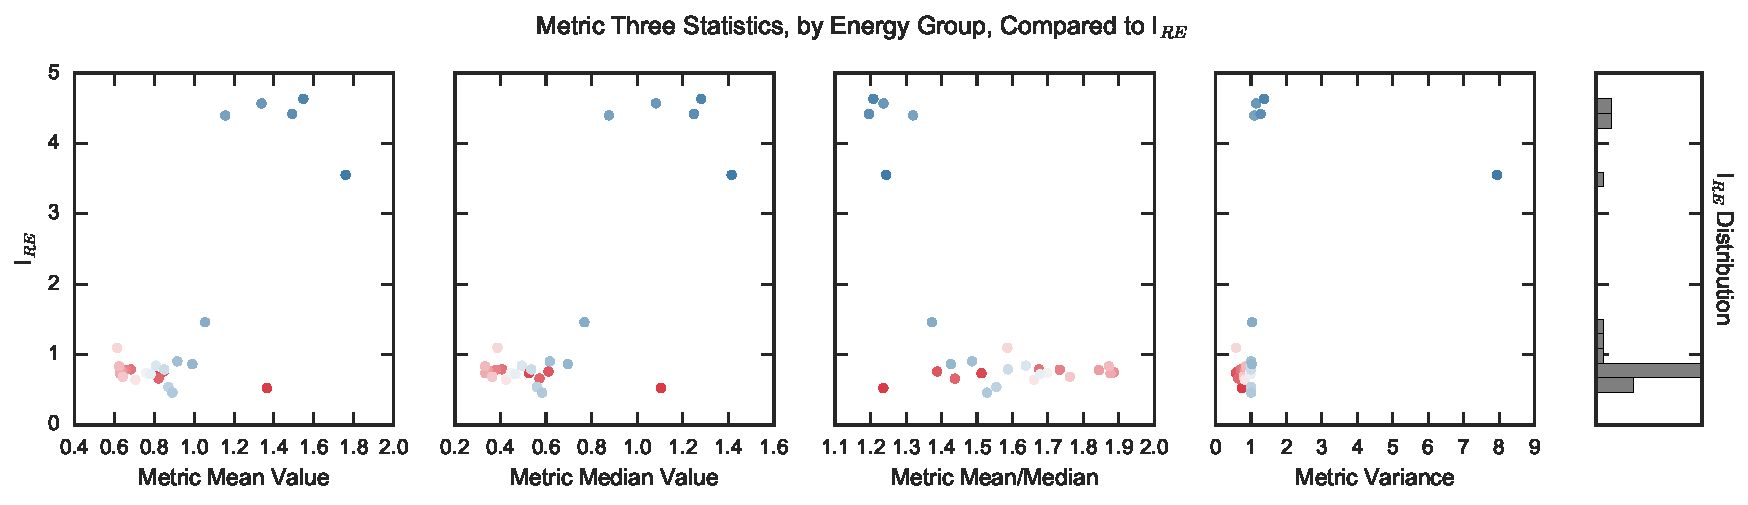
\includegraphics[width=\linewidth]{./chapters/characterization_probs/figures/sample_data/metric_three_err_stats_median.pdf}
    \caption{M$_3$ data selection above the metric median for each energy group,
      value average, mean, skew, and variance plotted against the
      relative error improvement I$_{RE}$}
    \label{fig:samplestatsmedianM3}
  \end{subfigure}
\end{figure}
\begin{figure}[htb!]\ContinuedFloat
  \centering
  \begin{subfigure}[t]{\textwidth}
    \centering
    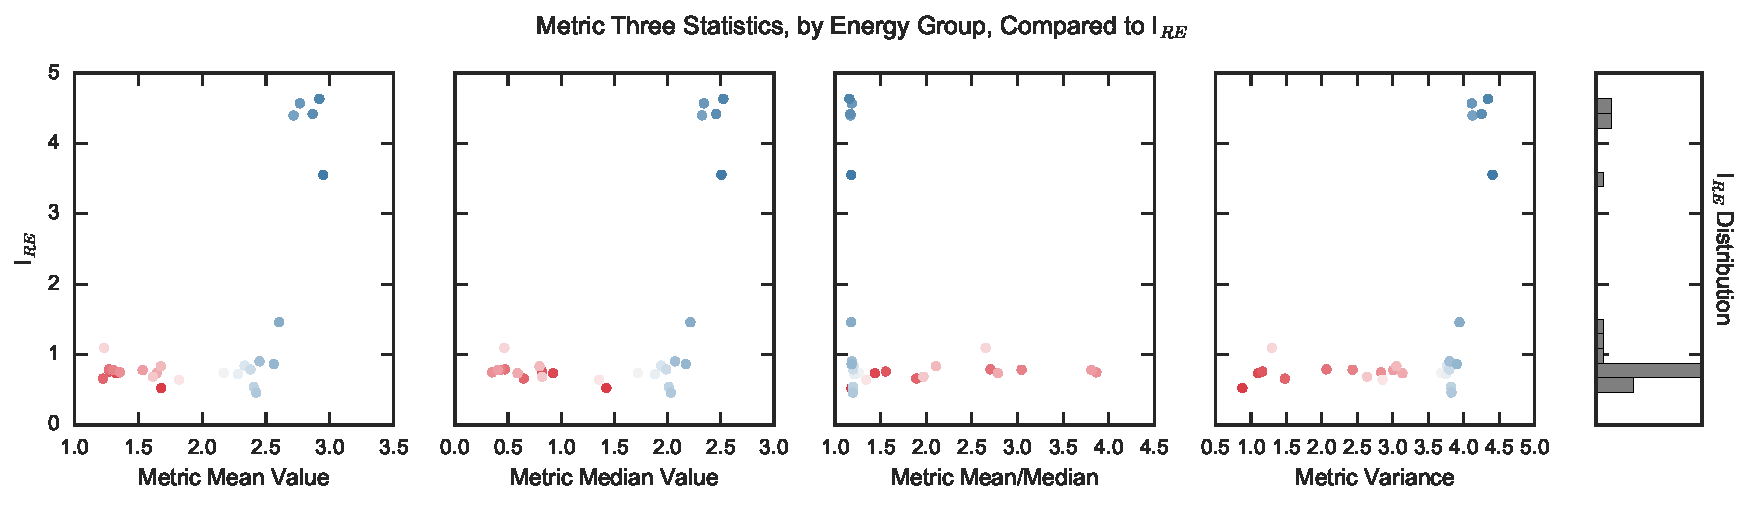
\includegraphics[width=\linewidth]{./chapters/characterization_probs/figures/sample_data/metric_three_err_stats_mean.pdf}
    \caption{M$_3$ data selection above the mean for each energy group,
      value average, mean, skew, and variance plotted against the
      relative error improvement I$_{RE}$ }
    \label{fig:samplestatsmeanM3}
  \end{subfigure}
  \caption[Sample scatterplots of M$_3$ distribution against the relative error
  improvement factor, I$_{RE}$.]
  {Sample scatterplots of the M$_3$ distribution against the relative error
    improvement factor, I$_{RE}$.}
  \label{fig:samplestats}
\end{figure}

There are several ways in which the improvement
factor I$_{RE}$ or I$_{FOM}$ may be compared against the anisotropy metrics. The
first are against the metric mean and median values. A plot of I versus either
of these values should look very simiar, with some shifting depending on the
distribution. However, if the mean and median are shifted significantly, this
would indicate a skew of the distribution. This skew may also be correlated with
either
of the I values. Last, it is possible that the spread of metric values may be
correlated with the I factor. Figure \ref{fig:samplestatsfullM3} is an
illustration of how I can be plotted with
each of these measurements of the metric distribution.

Similar to using the filtering algorithms in Figure
\ref{fig:sampleviolinsM2}, the data in the statistical trend plots can also be
filtered. The subfigures in \ref{fig:samplestats} illustrate how filtering out
the data by the contributon flux influences the location of I$_{RE}$ for each
energy group. Figure \ref{fig:samplestatsmedianM3} calculates the
metric mean, median, skew, and variance for each energy group using only metric
values in cells above the contributon median. Conversely, Figure
\ref{fig:samplestatsmeanM3} calculates the metric mean, median, skew, and
variance for each energy group using only metric values in cells above the
contributon median value.

The dots in each plot correspond to the same energy
groups plotted in \ref{fig:sampleviolinsM2}. That is, the lowest energy is
plotted in blue and the highest in red. Note that this type of plot is
possible because the Monte Carlo tally has been discretized to have
the same binning as the the deterministic code. It would be far more difficult
if the energy bin widths of the Monte Carlo tally did not match the
deterministic code.

The data that will be presented for each characterization problem
can be subdivided into three distinct
categories: data primarily obtained by the Monte Carlo calculation, data
primarily obtained by the deterministic calculation, and data that is a
combination of both. The FOM values using Monte Carlo runtimes, for example, is
in the first category. The anisotropy metrics presented in Section
\ref{sec:anisotropy_quant} are an example of a determinstic-exclusive dataset.
The results presented in Figure \ref{fig:samplestats} are a combination of both
deterministic and Monte Carlo-influenced results. In studying the $\Omega$
methods, we seek to understand how the $\Omega$ methods' performance influence
the Monte Carlo results. Beyond observing the FOM and relative error
distribution obtained in the Monte Carlo, the anisotropy metrics will provide
another avenue by which to investigate $\Omega$-method performance.

One may have deduced that the results for the characterization
problems and the subsequent angle
sensitivity study will be substantive. Only the most
pertinent fraction of the available data will be presented with each problem in
Sections \ref{sec:CharResults} and \ref{sec:AngleResults}. For example, in most
cases only a single figure--and perhaps only a single metric--from the
three presented in \ref{fig:samplestats}
will be presented for a particular problem, because only one will show a trend
relevant to the $\Omega$-methods' performance.
A more extensive set of data is accessible in Appendix \ref{ch:extended}; the
characterization problems will have extended results in Section
\ref{sec:extendedcharprobs} and the angle sensitivity study will be in
Section \ref{sec:extendedangle}.

